\documentclass[a4paper]{article}

\setlength{\oddsidemargin}{-4mm}
\addtolength{\topmargin}{-1in}
\addtolength{\footskip}{+0.5in}
\addtolength{\textwidth}{+1.5in}
\addtolength{\textheight}{+1in}

\usepackage[utf8]{inputenc}
\usepackage[english]{babel}
\usepackage{listings}
\usepackage{color}
\usepackage{multirow}
\usepackage{rotating}
\usepackage{graphicx}
\usepackage{caption}
\usepackage{amsmath}
\usepackage{subfig}

\renewcommand{\familydefault}{cmr}

\title{Report of Click Labs}
\author{Hong-Nam Hoang, Manh-Ha Nguyen and Xuan-Thu Thi Le}
\date{\today}

\begin{document}
  \maketitle
  \tableofcontents

  \definecolor{stringcolor}{rgb}{0.20,0.50,0.20}
  \definecolor{commentcolor}{rgb}{0.40,0.40,0.40}
  \definecolor{keywordcolor}{rgb}{0.50,0.10,0.10}
  \definecolor{idcolor}{rgb}{0.10,0.10,0.50}
  \definecolor{bg}{rgb}{0.95,0.95,0.95}  
  \lstdefinestyle{C}{basicstyle=\ttfamily,
                          keywordstyle=*\color{keywordcolor}\bfseries,
                          identifierstyle=\color{idcolor},
                          commentstyle={\color{black}\it},
                          stringstyle={\color{stringcolor}\ttfamily},
                          showstringspaces=false,
                          breaklines=true,
                          numbers=left,
                          numbersep=10pt,
                          stepnumber=1,
                          numberstyle=\small,
                          frame=single,
                          }

  \lstdefinelanguage[]{Click}[]{SQL}{
    morekeywords={elementclass, Counter, InfiniteSource, RateSource, Print, Paint, PaintSwitch, Script}}

  \section{Introduction}
  \section{ClickLabs package}
    \subsection{File organization}
      \begin{description}
      	\item[elements/] This directory contains all the additional click elements using in the lab.
      	\item[plot-template/] This directory contains templates used for plotting data by gnuplot. These files are used by draw-graph.sh
      	\item[bin/update-elements.sh] Run this file to update the new elements implemented in directory elements (above). For more information, type: ./update-elements.sh -h
      	\item[bin/visual-clicky.sh]Shell script to visualize click experiment using clicky. For more information, type: ./visual-clicky.sh -h
      	\item[bin/init.sh]Initialize Click environment for lab. Just run init.sh in the first time you get this source or click source directory changed.
      	\item[bin/eclick-compile.sh] Extend the Click file. A click file can include another one to reuse some compound elements (similar include in C, or import in Java). File eclick-compile.sh is used to translate (or flatten) these extended-click file to a normal click file.
      	\item[bin/convert-click-dump.sh]This script used to transform dump files from click (binary files) into text files. Note: this is one-way transformation, the binary files cannot be recovered from the text files.
      	\item[bin/draw-graph.sh] This script is used to draw graphs from data extracted in CLICK dump files. Just provide the dump files, this script will generate a graph for you. Note: No need to use convert-click-dump.sh before using draw-graph.sh.
      	\item[bin/draw-graph-framerelay.sh] Based on draw-graph.sh, this script helps to show the characteristics of verifying a conformance flow (which is deal with CIR, CBS, EBS).
      	\item[clicky.ccss] File supporting Clicky Cascading Style Sheets. It controls the appearance of a Clicky diagram with style sheets written in a CSS-like language.      	
      	\item[1-test-config/]
      	\item[2-tcp-udp-generation/]
      	\item[3-shaper-policer/]
      	\item[4-scheduler/]
      \end{description}
    
    \subsection{Some introductions before surfing Click configurations}
      \begin{enumerate}
      	\item 
      	  First of all, initialize the click environment for these stuffs. Run file init.sh: \\
      	    \texttt{chmod +x init.sh\\
      	    ./init.sh}\\
      	  Normally, init process takes long time for the first finding Click source path. To save time, you can create file \texttt{\~/.clickrc} with the content similar to this:\\
            \texttt{export CLICK\_SRC=/home/iizke/click/click-1.8.0}
        
        \item 
          While finishing to code some Click elements, put it in directory \texttt{elements}, and then run file \texttt{update-elements.sh} to compile and install new elements: \\
    \texttt{update-elements.sh}
        \item
        Explore the click configuration by using tool \texttt{visual-clicky.sh}. Simple way to use: \\    
    \texttt{visual-clicky.sh \$CLICK\_CONFIGURATION\_FILE}
        \item
        To support easy-reading and team-working activities, we developed a tool to allow including some click files into a click file. If you write some Click files as "\textit{library}" files, you can reuse it by using \textit{include statements}. For example, we have \texttt{TCP\_Source.click} to implement a TCP-generator, and \texttt{UDP\_Source.click} to implement an UDP-generator. In \texttt{TCP\_UDP.click}, we reuse the implementation of these generator by adding these lines at anywhere in \texttt{TCP\_UDP.click} file (but should be on the top for easy reading): \\
        \texttt{
  ------------------------ file: TCP\_UDP.click ---------------------------\\
  //#include "TCP\_Source.click"\\
  //#include "UDP\_Source.click"\\
  ...\\
  -------------------------------------------------------------------------}\\
  The syntax of include statement is simple:\\
          \texttt{//\#include "CLICK\_FILE\_PATH"}\\
  where \texttt{CLICK\_FILE\_PATH} can be relative or absolute path. After that, you have to use our tool (\texttt{eclick-compile.sh}) to pre-compile this file before simulating it by Click, for example:\\
    \texttt{eclick-compile.sh -o extend-TCP\_UDP.click [-f] TCP\_UDP.click}\\
Note: if using tool \texttt{visual-clicky.sh}, you don't have to pre-compile the extended-click file. It will do all automatically.
        \item To visualize your packet stream at input or output, we have developed \texttt{draw-graph.sh} to generate graph as picture (using \texttt{gnuplot} that should be installed before). The second, you have to provide the data. Normally, we usually generate data from Click with element \texttt{ToDump}. This data follows the tcpdump-like format. When you get the data, the last action you need is to run this command:\\
\texttt{draw-graph.sh -f dataIn.dump -f dataOut.dump \\
      $[$-o PNG\_FILES$]$\\
      $[$--plot-type COUNT (default) | RATE | DENSITY$]$\\
      $[$--xrange 233:23221$]$  $[$--yrange 282:2922$]$\\
      $[$--xlabel XYZ$]$  $[$--ylabel ABC$]$\\
      $[$--xcol 2$]$  $[$--ycol 1$]$}
      
  After program \texttt{draw-graph.sh} finishes its work, it will create a picture file (PNG file). If user does not use output option (-o), this program will export to screen (using default output file \texttt{/dev/output}). You may want to change the plotting template by modify files in \texttt{plot-template} directory.
      \end{enumerate}
  \section{Test configuration}
  In the first time of using Click, we try to implement \texttt{Counter\_test} element, \texttt{Random\_IP\_generator} element using basic Click elements, such as \texttt{Print, InfiniteSource, RatedSource, Script}, also trying to modify a part of source code of \texttt{InfiniteSource} to generate packets that randomize byte value at a specific location in payload.
  \subsection{\texttt{Counter\_test} Click configuration}
  \textbf{Location:} \texttt{1-test-config/Counter\_test.click} \\
  \begin{center}
	  \includegraphics[scale=0.6]{counter_test.pdf}
	  \captionof{figure}{\texttt{Counter\_test} Click configuration}
	  \label{fig:countertest}
  \end{center}
  To avoid IP CRC checking, we temporarily disable CRC checking by using flag "\texttt{CHECKSUM false}" in \texttt{CheckIPHeader} element. Another solution is to use \texttt{SetIPChecksum} to repair CRC in generated IP packets. Since we can visualize the result by using \texttt{clicky} to replace steps that print out screen counting results from \texttt{Counter} elements. 
  \subsection{\texttt{RandInfiniteSource} element}
  \textbf{Location:} \texttt{elements/randinfinitesource.*} \\
  This element is implemented by modifying source of \texttt{InfiniteSource} element. Its function is similar to \texttt{InfiniteSource}, but by adding one more keyword (\texttt{RNDBYTEID}), generated packets may have random byte value at a specified position in payload. The idea of implementation is that before pushing out packets to the output port, packet payload is changed. Originally, data packet is already prepared one time by \texttt{setup\_packet} function before \texttt{InfiniteSource} releases packets. To make new element work, after modifying data, \texttt{setup\_packet} function should be called, otherwise generated packets do not change their content. Figure \ref{fig:test-randsource} shows the result of using \texttt{RandInfiniteSource} element to generate five packets with random value at the first byte.
  \begin{center}
	\includegraphics[width=0.9\textwidth]{test-randinfinitesource.png}
	\captionof{figure}{Test \texttt{RandInfiniteSource} element with 5 packets and random at the first byte}
	\label{fig:test-randsource}
  \end{center}

  \subsection{\texttt{RandomQueue} element}
  There are two ideas of implementing Random Queue:
  \begin{itemize}
  	\item Random at input: Pushing packets at random positions in queue, but pulling out packets as FIFO queue. We try to simulate this behavior by using built-in Click elements.
  	\item Random at output: Pushing packets in type of FIFO, but pulling out random packets in queue. We have implemented new element called \texttt{RandomQueue}.
  \end{itemize}
  To test our element, we first generate a high rate packet at input, store current timestamps, let packet go through our elements to output which has lower rate than the input. We then print out packet timestamps to see whether they are random or not.
  \subsubsection{Using built-in Click elements (compound element)}
  \textbf{Location:} \texttt{1-test-config/randomqueue.click} \\
  We have implemented two versions:
  \begin{itemize}
  	\item \texttt{BRandomQueue} (we call it Binary Random Queue): \texttt{MixedQueue} allows us to put packets in type of FIFO (input port 0) or LIFO (input port 1). Based on this function, input packets are put randomly (by \texttt{RandomSwitch} element) in either FIFO or LIFO input port. By this way, if queue size is $n$, there are $2^n^-^1$ possibilities created over total possibilities $(n!)$. Technical issue: "When full, \texttt{MixedQueue} drops incoming FIFO packets, but drops the  oldest  packet to make room for incoming LIFO packets". It means that at that time, when observing at output, we only see packets with increasing timestamp, no randomly. We resolve this problem by writing a script to drop LIFO packet when queue is full.
  	\item \texttt{2PRandomQueue} (Two Partition Random Queue): We expand the above idea with two queues and using Stride scheduler to join them to the output. Note that, dropped packets in the first queue are push to the second queue.
  \end{itemize}
  \begin{figure}[ht]
      \centering
      \subfloat[\texttt{BRandomQueue}]{
      \label{fig:brandomqueue}
      \includegraphics[width=0.8\textwidth]{brandomqueue.pdf}}
      
      \subfloat[\texttt{2PRandomQueue}]{
      \label{fig:2prandomqueue}
      \includegraphics[width=0.8\textwidth]{2prandomqueue.pdf}}
      
      \caption{Random Queue configurations based on built-in Click elements}
      \label{fig:clickrandomqueue}
  \end{figure}
  
    \begin{figure}
      \centering
      \subfloat[\texttt{BRandomQueue}]{
      \label{fig:test-brandomqueue}
      \includegraphics[width=0.35\textwidth]{test-brandomqueue.png}}      
      \subfloat[\texttt{2PRandomQueue}]{
      \label{fig:test-2prandomqueue}
      \includegraphics[width=0.3\textwidth]{test-2prandomqueue.png}}
      \caption{Test results of Random Queue configurations}
      \label{fig:test-clickrandomqueue}
  \end{figure}
  
  \subsubsection{Writing new element: \texttt{RandomQueue}}
  \textbf{Location:} \texttt{elements/randomqueue.*} \\
  This element is inherited from \texttt{ThreadSafeQueue} class. We reuse all the source code but modifying the \texttt{pull} function to make it pull out packets randomly. Since queue data structure is not suitable for pulling out random packet (only good for the head and tail packets), we use a trick that swapping the random packet and the first packet. Step by step in our algorithm as following:
  \begin{center}
	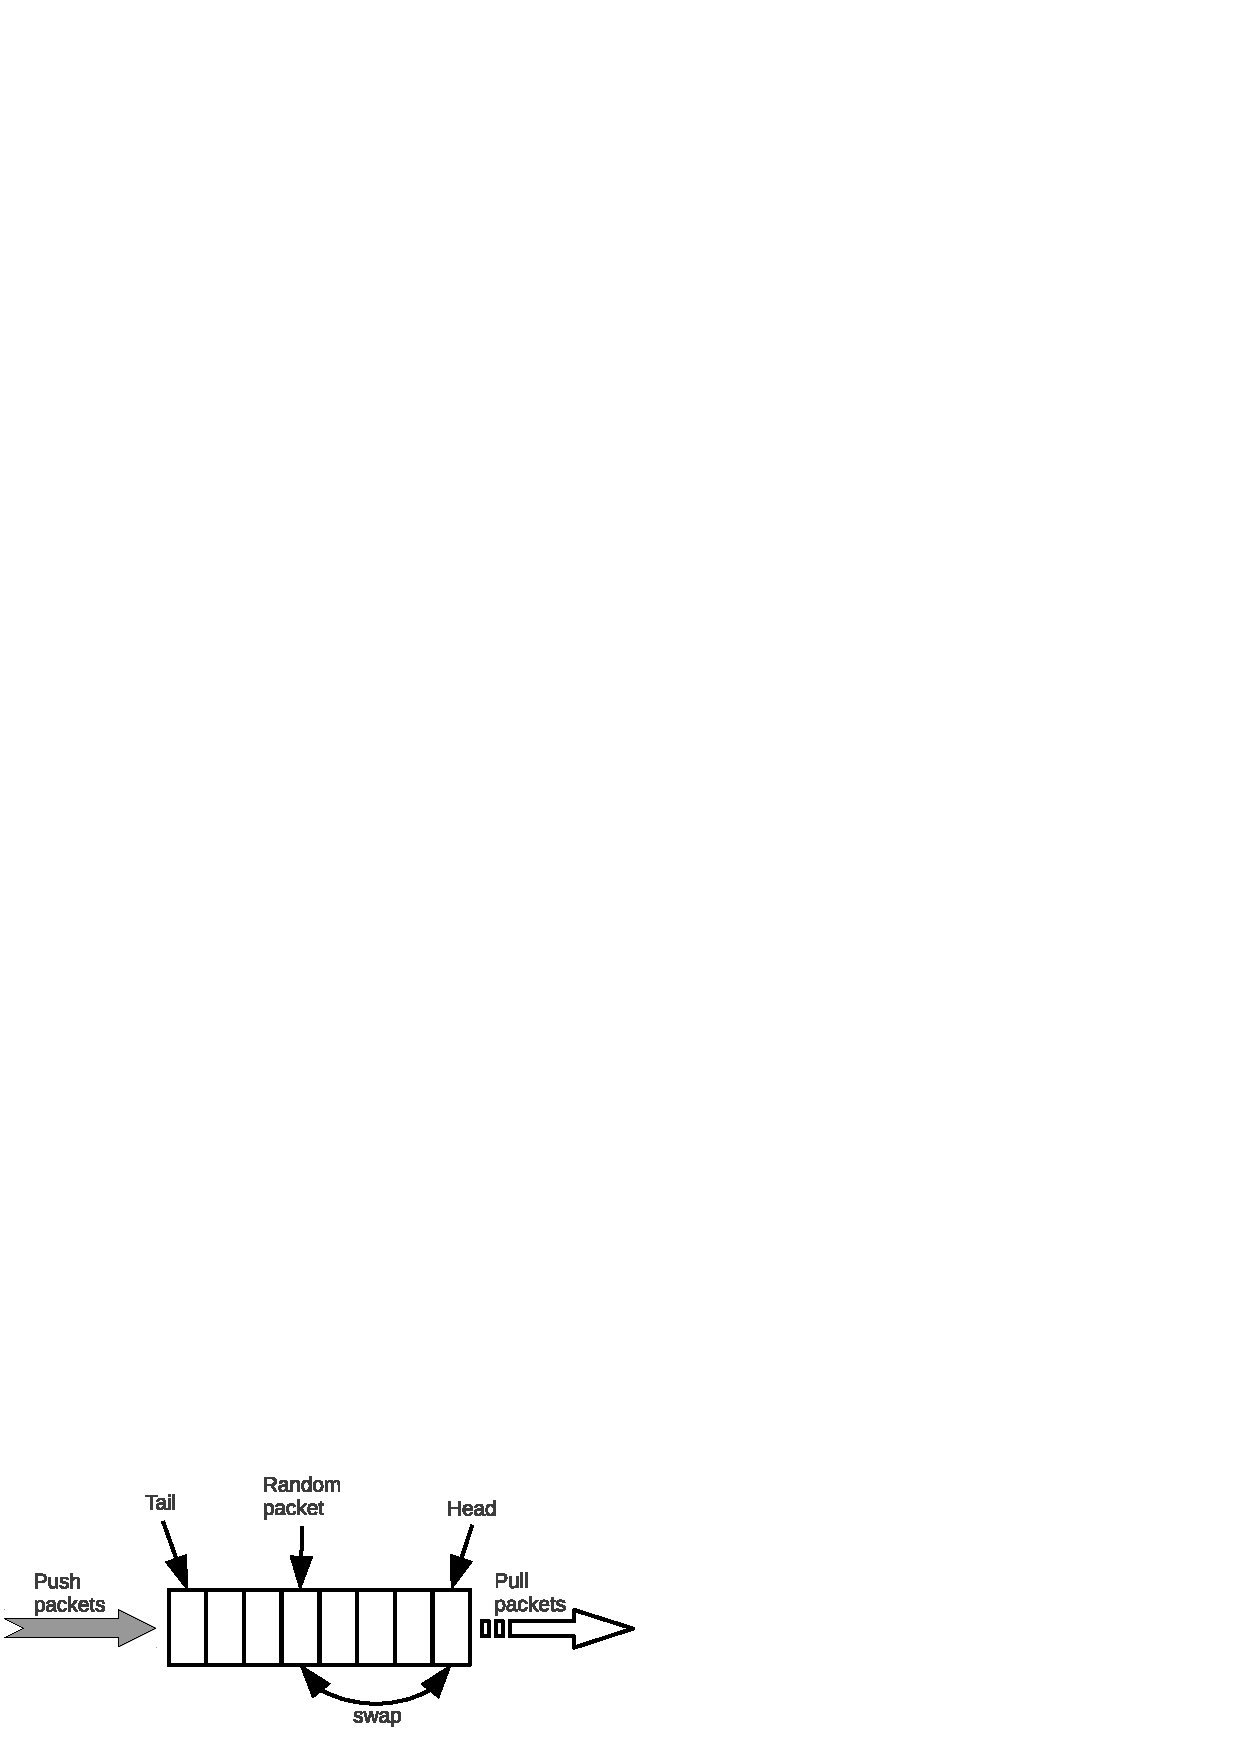
\includegraphics[scale=0.80]{randomqueue-alg.pdf}
	\captionof{figure}{Behavior of \texttt{RandomQueue} element}
	\label{fig:randomqueue}
  \end{center}

  \begin{itemize}
  	\item First, determining which packet is pulled out by a random number in the range from $0$ to \texttt{RandomQueue.length}.
  	\item Next, swapping the random packet and the first packet.
  	\item Last, pull out the first packet (but actually the random packet).
  \end{itemize}
  \begin{center}
	\includegraphics[scale=0.70]{test-randomqueue.png}
	\captionof{figure}{Test \texttt{RandomQueue} element}
	\label{fig:test-randomqueue}
  \end{center}

  \subsection{\texttt{Random\_IP\_generator} configuration}
  \textbf{Location:} \texttt{1-test-config/Random\_IP\_generator.click} \\
  We combine \texttt{RandInfiniteSource, RandomQueue} with other elements to build this configuration:
  \begin{itemize}
   	\item \texttt{RandInfiniteSource}: generate packets with random source IP address in the form 192.168.1.x. In this situation, we set up "RNDBYTEID 30".
   	\item \texttt{RandomQueue}: pull out packets at random position in queue. We can replace \texttt{RandomQueue} to another types of queue, such as FIFO or LIFO, by using \texttt{MixedQueue} element (comment lines in \texttt{Random\_IP\_generator} configuration). 
   	\item \texttt{SetCRC32, CheckCRC32}: set or check CRC32.
   	\item \texttt{RandomBitError}: to simulate an error free link via a queue element.
   	\item \texttt{Script}: we add some scripts to check states: 
       	\begin{itemize}
       		\item \texttt{autoupdate\_lostp\_estimation}: calculation based on bit error from \texttt{RandomBitError} and number of 'input' packets (\texttt{c1} in figure \ref{fig:randomipgenerator}).
       		\item \texttt{autoupdate\_real\_bit\_error}: based on \texttt{c1, c2}. 
       		\item \texttt{autoupdate\_lostp\_percent}: based on \texttt{c1, c2}.
       	\end{itemize}
   \end{itemize} 
  \begin{center}
	  \includegraphics[scale=0.55]{Random_IP_generator.pdf}
	  \captionof{figure}{\texttt{Random\_IP\_generator} configuration}
	  \label{fig:randomipgenerator}
  \end{center}
  \section{TCP/UDP traffic generation}
  \subsection{TCP traffic}
  \textbf{Location:} \texttt{2-tcp-udp-generation/TCP\_Source.click} \\
  The procedure of generating TCP packet as following:
  \begin{itemize}
  	\item First, we use \texttt{TimedSource} to generate TCP packet without IP header.
  	\item After that, this packet is encapsulated IP header by \texttt{IPEncap}. Remember to setup "PROTO 0x06" to say that it is TCP packet.
  	\item Encapsulate ethernet header with "ETHERTYPE 0x0800" in each packet.
  \end{itemize}
  \begin{center}
	  \includegraphics[scale=0.55]{TCP_Source.pdf}
	  \captionof{figure}{\texttt{TCP\_Source} element}
	  \label{fig:tcpsource}
  \end{center}
  \subsection{UDP traffic}
  \textbf{Location:} \texttt{2-tcp-udp-generation/UDP\_Source.click} \\
  \texttt{UDP\_Generator} operates like \texttt{TCP\_Generator}. Note: when using \texttt{IPEncap}, setup "PROTO 0x11" for UDP packet.
    \begin{center}
	  \includegraphics[scale=0.55]{UDP_Source.pdf}
	  \captionof{figure}{\texttt{UDP\_Source} element}
	  \label{fig:udpsource}
  \end{center}
  \subsection{\texttt{TCP\_UDP\_generator} configuration}
  \textbf{Location:} \texttt{2-tcp-udp-generation/TCP\_UDP\_generator.click} \\
  We build this configuration as in figure \ref{fig:tcpudp}. TCP source is created with rate about 1000 packets per second (pps) while UDP packet rate is 1 pps. Script \texttt{autoupdate\_scale} is used to check online the ratio between number of TCP packets and number of UDP packets. We see that this generator works well when both queues are not full or speed of output link (\texttt{TimedSink}) is very fast. When queues are full, the expected ratio is not guaranteed. At our observation, we try to formalize the ratio as following:
  \begin{itemize}
  	\item Let $r_{tcp}$, $r_{udp}$, $r$ are respectively the rate of TCP source, UDP source and output link. Let $ratio$ is the ratio between number of TCP packets over number of UDP packets at output link.
  	\item Let $R = (r_{tcp} + r_{udp})$, and $m = \min(r_{tcp}, r_{udp})$.
  	\item If $r \ge R$: $ratio = \frac{r_{tcp}}{r_{udp}}$
  	\item If $r \le 2m$: $ratio = 1$
  	\item If $ 2m < r < R$: $ratio = \frac{m}{r - m}$
  \end{itemize}
  In general, we have a formular of ratio like: $ratio = \frac{m}{\min(R, \max(2m, r)) - m}$.
    \begin{center}
	  \includegraphics[scale=0.4]{TCP_UDP_generator.pdf}
	  \captionof{figure}{\texttt{TCP\_UDP\_generator} configuration}
	  \label{fig:tcpudp}
  \end{center}
  \section{Shapers and Policers}
  In this part, we implement elements with consideration at packet level, not byte level.
  \subsection{Uncontrolled flow}
  \textbf{Location:} \texttt{3-shaper-policer/uncontrol-flow.click} \\
  We have tried some implementations of uncontrolled flow but the main idea is that the inter-time (interval) between two consecutive packets is a random
  number. All implementations of uncontrolled flow are put in \texttt{3-shaper-policer/uncontrol-flow.click}. Normally, we use \texttt{RatedSource} or \texttt{TimedSource} to generate packets at a specific rate. After some time, we use Script to change their rate or interval at a random values. We list here with a few lines of description of each implementation:
  \begin{itemize}
  	\item \texttt{UncontrolledFlow0}: We use two rated sources, one for generating regular rated source, one for generating burst. These sources are connected to a pull switch to choose from which source packets are generated. At any time generating packets, we choose a source to generate next packets through a script. 
  	\item \texttt{UncontrolledFlow1}: Only one source (\textt{InfiniteSource}) is used and connected directly to the output. We used another two scripts named \texttt{change\_rate} and \texttt{autoupdate\_change\_burst} to change rate and burst at runtime.
  	\item \texttt{SimpleUncontrolledFlow}: we use \texttt{RatedSource} instead of \textt{InfiniteSource} and one script to change the rate of source each one second. Script operates in type ACTIVE.
  	\item \texttt{ProbUncontrolledFlow} (Figure \ref{fig:probuncontrolledflow}): similar to \texttt{SimpleUncontrolledFlow} but change-rate script operates in type PACKET. When one packet go through this script, it will decide whether rate of source is changed or not based on a probability defined by user.
  	\item \texttt{BurstUncontrolledFlow}: We use eight sources (\texttt{RatedSource}), all connected to a \texttt{ThreadSafeQueue}. At each source, packets can be dropped at a defined probability. As a result, this compound element generates packets at a particular rate but random burst (maximum burst size is 8). 
  \end{itemize}
  \begin{center}
	\includegraphics[width=0.60\textwidth]{probuncontrolledflow.pdf}
	\captionof{figure}{Uncontrolled flow with probability of changing rate source.}
	\label{fig:probuncontrolledflow}
  \end{center}
  
  \subsection{Leaky bucket}
  \textbf{Location:} \texttt{3-shaper-policer/leaky-bucket.click} \\
  Since leaky bucket does not admit any burtiness, we design the leaky bucket policer with a queue of size 1 (maximum 1 packet in a queue at a time) (figure \ref{fig:test-leaky}). After that, we use \texttt{RatedUnqueue} or \texttt{TimedSource} to create CBR source. We use both these elements because of a technical issue: when the rate is less than 1000 packets/second, \texttt{RatedUnqueue} can release packets from queue with burstiness. So, at the beginning of starting leaky policer, the \texttt{Init} script will decide which one of unqueue elements is used.
  \begin{center}
	\includegraphics[width=1.0\textwidth]{leaky-shaper.pdf}
	\captionof{figure}{Leaky bucket configuration (policer and shaper)}
	\label{fig:test-leaky}
  \end{center}
  Scenario of testing leaky bucket: \texttt{ProbUncontrolledFlow} is the source of packets with maximum rate 1000 pps (packets per second). The leaky policer only allows 400 pps. Shaper of leaky bucket uses a buffer of 2000 packets and generate packets from buffer at rate 400pps to the leaky policer. Figure \ref{fig:test-leakypolicer-graph} shows that the number of output packets is linear to time although the input is not.  
  \begin{center}
	\includegraphics[width=0.8\textwidth]{leaky-count.png}
	\captionof{figure}{Monitor number of packets at input (uncontrolled flow) and output of leaky policer and shaper}
	\label{fig:test-leakypolicer-graph}
  \end{center} 
  
  \subsection{Token bucket}
  \textbf{Location:} \texttt{3-shaper-policer/token-bucket.click} \\
  Token bucket is designed similar to leaky bucket but expand the size of queue as a number of burstiness, see \texttt{RatedTokenBucketPolicer3} in figure \ref{fig:test-token}. But before implementing this element, there are some alternative implementations which are more complex:
  \begin{itemize}
  	\item \texttt{RatedTokenBucketPolicer1}: We use a variable-size queue in this element. The size of queue is increase with the rate that is equal to the rate of token bucket. Each time a packet goes out of queue, the capacity of queue is decrease one. 
  	\item \texttt{RatedTokenBucketPolicer2}: This element use a sample source (same rate as token bucket, operating as a token generator) and two counter to count the number of output packets ($CI$) and the number of generated token packets ($CT$). This element guarantees that: $CI \le CT \le CI + burst$. If this condition is satisfied, input packets are pushed to output immediately, otherwise they are dropped. This element releases packets to output as soon as possible (there is no queue to store input packets) while other implementations try to store input packets first and then regulate the output flow at a specific rate.
  \end{itemize} 
  \begin{center}
	\includegraphics[width=1.0\textwidth]{token-shaper.pdf}
	\captionof{figure}{Token bucket configuration \texttt{RatedTokenBucketShaper3}}
	\label{fig:test-token}
  \end{center}
  
  \begin{center}
	\includegraphics[width=0.8\textwidth]{token-count.png}
	\captionof{figure}{Monitor number of packets at input (uncontrolled flow) and output of token policer and shaper}
	\label{fig:test-tokenpolicer-graph}
  \end{center} 

  Figure \ref{fig:test-token-leaky-graph} does a comparison of token and leaky bucket. The scenario is: we try to regulate a \texttt{BurstUncontrolledFlow}  (rate is 1 pps and maximum burst is 8) by a token and a leaky bucket policer. Token bucket policer is \texttt{RatedTokenBucketPolicer3} (rate is 10 pps, burst is 10), and leaky policer is \texttt{RatedLeakyBucketPolicer} (rate is 10 pps). We see that token policer can allow some burstiness but leaky policer limits the burstiness.
  \begin{center}
	\includegraphics[width=0.8\textwidth]{compare-lk-tk.png}
	\captionof{figure}{Comparision of Token bucket and Leaky bucket}
	\label{fig:test-token-leaky-graph}
  \end{center} 
  
  \subsection{Cascading Leaky and Token bucket}
  If leaky bucket is put before token bucket, the token policer donot have to take care of burstiness but only the rate of flow.
  If token bucket is put before leaky bucket, the leaky policer will not allow burstiness from token policer or shaper if rate of leaky is smaller than the peak rate of token.  
  \subsection{Negotiation (CIR, CBS, EBS)}
  \textbf{Location:} \texttt{3-shaper-policer/negotiation.click} \\
  Figure \ref{fig:negotiation} shows one implementation of negotiation. The idea is: packets are classified into low and high priority. Packet is high priority and put into \texttt{HighQueue} if there is free space in \texttt{HighQueue} (capacity $CBS$), otherwise it is in \texttt{LowQueue} (capacity $EBS$) with low priority. Since rate $CIR$ is fixed, the window time $T = \frac{CBS}{CIR}$ is scale to $CIR$. We use a counter \texttt{TimeCount} to know when the window time is end (by observing $\texttt{TimeCount} = CBS$). If this happens, we reset all the counters for a new window time. Since we calculate the window time base on $CBS$, we have to make sure that there are always packets to \texttt{TimeCount} at rate $CIR$. So, we use \texttt{SampleSource} generating packets at rate $CIR$ and \texttt{PrioScheduler} to guarantee that condition. At output, there are only $(CBS+EBS)$ packets in a window time $T$. The high priority packets are on port 0, and the low priority packets are on port 1.
  \begin{center}
	\includegraphics[width=0.80\textwidth]{negotiation.png}
	\captionof{figure}{One implementation of negotiating CIR, CBS, EBS}
	\label{fig:negotiation}
  \end{center}
  Figure \ref{fig:negotiation-check} shows a testing result with \texttt{RatedNegotiablePolicer3\_1}.
    \begin{figure}
    \centering
    \includegraphics[width=0.80\textwidth]{negotiation-check.png}
	  \captionof{figure}{Number of packets in a time $CBS/CIR$}
	  \label{fig:negotiation-check}
    \end{figure}

  \subsection{Generic Cell Rate Algorithm - GCRA}
  \textbf{Location:} \texttt{3-shaper-policer/gcra.click} \\
  
  \begin{center}
	\includegraphics[width=0.80\textwidth]{gcra.pdf}
	\captionof{figure}{\texttt{GCRA} configuration}
	\label{fig:gcra}
  \end{center}
  
  \begin{center}
	\includegraphics[width=0.80\textwidth]{test-gcra.png}
	\captionof{figure}{Testing GCRA configuration with flow \texttt{ProbUncontrolledFlow}}
	\label{fig:test-gcra}
  \end{center}
  
  \section{Schedulers}
  \subsection{FIFO scheduler}
  There are two ways of building FIFO scheduler. The first and simple way is to use \texttt{ThreadSafeQueue} element. All inputs are connected into input of queue and output of queue is connected to output of FIFO scheduler. The second way is to use \texttt{TimeSortedSched} element to which all inputs connect through queues. 
  \begin{center}
	\includegraphics[width=0.80\textwidth]{fifo-dense.png}
	\captionof{figure}{Testing \texttt{FIFOSched} configuration}
	\label{fig:test-fifo}
  \end{center}
  
  \subsection{Round Robin scheduler}
  Round Robin Scheduler is built-in element in Click. 
  \begin{center}
	\includegraphics[width=0.80\textwidth]{rr-dense.png}
	\captionof{figure}{Testing \texttt{RRSched} configuration}
	\label{fig:test-rr}
  \end{center}
  
  \subsection{Deficit Round Robin scheduler}
  Deficit Round Robin Scheduler is built-in element in Click. 
  \begin{center}
	\includegraphics[width=0.80\textwidth]{drr-dense.png}
	\captionof{figure}{Testing \texttt{DRRSched} configuration}
	\label{fig:test-drr}
  \end{center}
  
  \subsection{Weighted Round Robin Scheduler}
  We implement this scheduler in two versions. The first is compound elements that based on Round Robin scheduler. The second is a new element.
  \subsubsection{WRR scheduler - compound element}
  This scheduler is based on Round Robin scheduler. The main idea is that: weight of each flow is scaled to number of ports assigned to that flow. A high weight flow will have more input ports of Round Robin scheduler. In practice, we need to take care of distribution of ports to have the fairness in response time.
  \begin{center}
	\includegraphics[width=0.80\textwidth]{wrr2-dense.png}
	\captionof{figure}{Testing \texttt{WRRSched} compound element}
	\label{fig:test-wrr-compound}
  \end{center}
  
  \subsubsection{WRR scheduler - new element}
  Since WRR compound element is not easy to deal with big weight although only a few number of inputs, we developed a new element for WRR scheduler. $N$ is number of input, $w_i$ is weight of $i$-th input, $W$ is total of weights. At initial time, this element will create a list of visited ports in period of $W$ steps, and try to make fairness in response time.
  \begin{center}
	\includegraphics[width=0.80\textwidth]{wrr-dense.png}
	\captionof{figure}{Testing \texttt{WRRSched} element}
	\label{fig:test-wrr}
  \end{center}

  \subsection{Weighted Deficit Round Robin scheduler}
  Not implement as a new Click element but only a compound element, similar to the compound element of WRR scheduler.
  \subsection{\texttt{SetVirtualClock} element}
  It is a new Click element which is used to support Virtual Clock scheduler and Weighted Fair Queue scheduler. Its important feature is the ability of remembering the last computed value. Each time a packet arrives, it will set a new virtual time (tag) into timestamps annotation of packet. 
  \subsection{Virtual Clock scheduler}
  \begin{center}
	\includegraphics[width=0.80\textwidth]{test-vcsched.pdf}
	\captionof{figure}{\texttt{VirtualClock} scheduler with 3 flows}
	\label{fig:vcsched}
  \end{center}
 
  \begin{center}
	\includegraphics[width=0.80\textwidth]{vcs-dense.png}
	\captionof{figure}{Testing \texttt{VirtualClock} scheduler with 3 flows}
	\label{fig:test-vcs}
  \end{center}
 
  \subsection{Weighted Fair Queue scheduler}
  \section{Congestion control}
    \begin{center}
	  \includegraphics[scale=0.5]{wred2.pdf}
	  \captionof{figure}{One simple implementation of \texttt{WRED} element}
	  \label{fig:wred2}
    \end{center}
  
\end{document}
